\setcounter{ExampleCounter}{1}
To begin our study of logic, we must first define our most basic unit, the \textbf{statement}; we'll consider whether specific statements are true or not, and we'll combine statements to form compound statements and ultimately arguments.

The following sentences are statements:
\begin{center}
It rained yesterday.\\
The Packers will win the Super Bowl this year.\\
Elephants are afraid of mice.
\end{center}

\begin{proc}{Statements}
A \textbf{statement} is a claim that is either true or false, but not both.
\end{proc}

Notice that it doesn't matter for the definition whether we know if a statement is true or false; it simply has to be one or the other.\\

What, then, is not a statement?  The following are a few examples:
\begin{center}
Get some milk at the store.\\
Why is the sky blue?\\
This sentence is false.
\end{center}
The first is a command and the second is a question, neither of which have any claim to being true or false.  It doesn't make sense to talk about truth values with them.

The third is an interesting one.  At first, it looks like a statement, because it makes a claim; however, upon closer inspection, we see that it isn't either true or false.  This is known as the \textit{liar's paradox}: if it were true, it would be false, which would mean it is true, which would mean...\\

In this chapter, we will commonly represent statements with letters to shorten the amount we have to write.  For instance, we might define\footnote{We typically start with $p$ for \textit{proposition}, another name for a statement} $p$ and $q$ as
\begin{center}
$p$: Today is the longest day of the year.\\
$q$: Tomorrow is the shortest day of the year.
\end{center}
That way, if we want to combine these statements, we don't have to write them out over and over again; we can simply write $p$ and $q$ and save a lot of trouble.\\

In the coming sections, we'll spend a lot of time combining statements in various ways, and it can be easy to get lost in the notation and think of logic as some sort of abstract study of notation.  Resist this temptation.  Instead, always remember that the letters and symbols we use and manipulate are tied to simple statements like these examples.  With every new operation we investigate, our goal is to not just focus on memorizing a list of symbols, but rather to understand why this operation makes sense.

\subsection{Boolean Logic with Sets}
Every time you use Google to search the Internet, the search engine turns to Boolean logic to narrow down the search results to give you what you're looking for, using key terms like ``and,''\marginnote{Three basic Boolean operators:\\
\begin{enumerate}
\item And
\item Or
\item Not
\end{enumerate}} ``or,'' and ``not.''

For instance, if you searched for ``Frederick,'' the search engine would pull up results that contain that word (like the city tourism website, the Wikipedia article on the city, maybe the article for Frederick Douglass, etc.).  If you searched for ``Frederick Community College,'' the search engine would look for pages that contain those three words; it would search for ``Frederick'' AND ``Community'' AND ``College.''

If instead you search for ``Frederick Community $-$College,'' the search engine will search for pages that contain ``Frederick'' AND ``Community'' but NOT ``College,'' so the FCC website will not be listed.\\

We can think of objects as belonging to sets; in this case, performing a search means looking for objects that belong to a specific list of sets.  For instance, if you went to library and searched ``History'' AND ``Fiction,'' you would find all the books that belong both to the History set and to the Fiction set (i.e. historical fiction).
\vfill
\pagebreak

As it turns out, we can deal with logic using either statements or sets.  When working with statements, Boolean logic combines multiple statements that are either true or false into a compound statement that is either true or false.  When working with sets, Boolean logic combines sets, and a search is considered ``true'' when it returns an object in that combination of sets.
\begin{center}
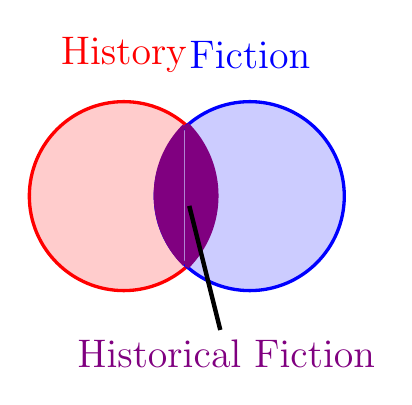
\begin{tikzpicture}
  \draw [very thick,color=red, fill=red!20] (-0.8,0) circle (1.2cm);
  \draw [yshift=1.8cm,xshift=-0.8cm] node {\color{red}\Large History};
  
  \draw [very thick,color=blue, fill=blue!20] (0.8,0) circle (1.2cm);
  \draw [yshift=1.8cm,xshift=0.8cm] node {\color{blue}\Large Fiction};
  
  \draw [yshift=-2cm,xshift=0.5cm] node (a) {\color{blue!50!red}\Large Historical Fiction};
  \draw [yshift=0cm,xshift=0cm] node (b) {};
  
  \draw [ultra thick,color=blue!50!red, fill=blue!50!red] (0,-0.9) arc (-45:45:1.28cm);
  \draw [ultra thick,color=blue!50!red, fill=blue!50!red] (-0.03,0.89) arc (135:225:1.24cm);
  \draw [ultra thick,color=blue!50!red] (0,-0.9) -- (0,0.9);
  
  \draw [ultra thick] (a) -- (b);
\end{tikzpicture}
\end{center}

We can draw similar diagrams for the other two basic Boolean operations.  For instance, if we searched for ``History'' OR ``Fiction,'' the search would return any books that are either historical or fiction, or both.
\begin{center}
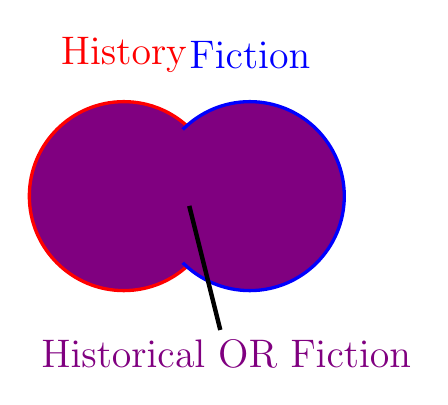
\begin{tikzpicture}
  \draw [very thick,color=red, fill=blue!50!red] (-0.8,0) circle (1.2cm);
  \draw [yshift=1.8cm,xshift=-0.8cm] node {\color{red}\Large History};
  
  \draw [very thick,color=blue, fill=blue!50!red] (0.8,0) circle (1.2cm);
  \draw [yshift=1.8cm,xshift=0.8cm] node {\color{blue}\Large Fiction};
  
  \draw [yshift=-2cm,xshift=0.5cm] node (a) {\color{blue!50!red}\Large Historical OR Fiction};
  \draw [yshift=0cm,xshift=0cm] node (b) {};
  
  \draw [ultra thick,color=blue!50!red, fill=blue!50!red] (-0.8,-1.1) arc (-90:90:1.1cm);
  
  \draw [ultra thick] (a) -- (b);
\end{tikzpicture}
\end{center}

This is what is called the \textit{inclusive} OR; it includes all values in the first set, plus all values in the second set, plus all values in the overlap.  There is also an \textit{exclusive} OR operation (that we won't consider) that includes all values in the first set and all values in the second set, but \textit{not} the values in the overlap.  It is equivalent to saying ``Either history or fiction, but not both.''

The inclusive OR is like the following question at a restaurant: ``Would you like fries or a drink with that?''  It is perfectly acceptable to respond ``Both, please.''\\

Finally, if we searched for NOT ``Fiction,'' the search\footnote{For obvious reasons, Google gives an error if you only search for NOT something} would return everything in the database except for those labeled ``Fiction.''\\

\begin{center}
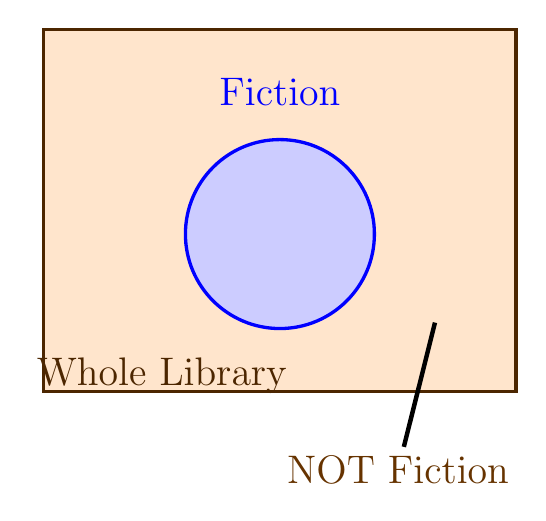
\begin{tikzpicture}
  \draw [very thick,color=orange!30!black, fill=orange!20] (-3cm,-2cm) rectangle (3cm,2.6cm);

  \draw [very thick,color=blue, fill=blue!20] (0,0) circle (1.2cm);
  \draw [yshift=1.8cm,xshift=0cm] node {\color{blue}\Large Fiction};
  
  %\draw [very thick,color=blue, fill=blue!20] (0.8,0) circle (1.2cm);
  %\draw [yshift=1.8cm,xshift=0.8cm] node {\color{blue}\Large Fiction};
  
  \draw [yshift=-3cm,xshift=1.5cm] node (a) {\color{orange!40!black}\Large NOT Fiction};
  \draw [yshift=-1cm,xshift=2cm] node (b) {};
  \draw [yshift=-1.8cm,xshift=-1.5cm] node {\color{orange!30!black}\Large Whole Library};
  
  %\draw [ultra thick,color=blue!50!red, fill=blue!50!red] (0,-0.9) arc (-45:45:1.28cm);
  %\draw [ultra thick,color=blue!50!red, fill=blue!50!red] (-0.03,0.89) arc (135:225:1.24cm);
  %\draw [ultra thick,color=blue!50!red] (0,-0.9) -- (0,0.9);
  
  \draw [ultra thick] (a) -- (b);
\end{tikzpicture}
\end{center}

Diagrams like these will helpful to visualize combining statements using these three operations.
\pagebreak

\begin{example}[https://www.youtube.com/watch?v=E_BhHaTb1pw]{Search Logic}
Suppose we are searching for universities in Mexico.  Express a reasonable search using Boolean logic.

\sol
We could search for ``Mexico AND university,'' but we would be likely to get results for universities in New Mexico (in the U.S.).  To account for this, we could revise our search terms:
\begin{center}
Mexico AND university NOT ``New Mexico''
\end{center}
The quotes around New Mexico group those words together, so that the search engine will know that we want to exclude that \textit{string}.\\

Also, in most search engines, including the word AND is unnecessary, since the search engines that if you provide two keywords, you want results that include both keywords.  In Google, a negative sign in front of a terms is used to indicate NOT.\\

Thus, in Google, this search would be
\begin{center}
Mexico university $-$``New Mexico''
\end{center}
\end{example}

\begin{example}[https://www.youtube.com/watch?v=G-1JBcYqz_o]{Describing a Set}
Describe the set of numbers that meet the following conditions:
\begin{center}
Even numbers that are greater than 12 and less than 20.
\end{center}

\sol
We could describe this as ``numbers that are even'' AND ``numbers that are greater than 12'' AND ``numbers that are less than 20,'' so we're looking for the overlap for these three sets.\\

The numbers that fit this description are \[\boxed{\{14,16,18\}}\]
\end{example}

\subsection{Boolean Logic with Statements}
We can use these same three operators with statements; instead of thinking of objects belonging to sets, we'll think about whether statements are true or false.\\

For instance, consider the following two statements.
\begin{center}
$p$: Greece belongs to the European Union.\\
$q$: Tokyo is in Iran.
\end{center}

Clearly, $p$ is true and $q$ is false.  What about $p$ AND $q$?  In words, this would be the compound statement ``Greece belongs to the European Union, and Tokyo is in Iran.''  

\begin{proc}{Combining Statements with AND}
The compound statement $p$ AND $q$ is only true if $p$ and $q$ are both true; if either one is false, that makes the compound statement false.
\end{proc}

In this example, the fact that $q$ is false makes the compound statement break down; just because the first half is true isn't enough.

On the other hand, what if we wrote ``Greece belongs to the European Union or Tokyo is in Iran''?  In this case, the fact that the first half is true is enough to satisfy the compound statement.

\begin{proc}{Combining Statements with OR}
The compound statement $p$ OR $q$ is true if at least one of $p$ and $q$ are true.
\end{proc}

Therefore, $p$ OR $q$ is true, simply because $p$ is true.\\

Finally, what about NOT, the last of the three basic Boolean operators?  What if we wrote ``Greece does not belong to the European Union''?  This statement would be false, because it is the opposite of a true statement.  Conversely, ``Tokyo is not in Iran'' would be true, because it is the opposite of a false statement.

\begin{proc}{Negating Statements with NOT}
If $p$ is true, then NOT $p$ is false; if $p$ is false, then NOT $p$ is true.
\end{proc}

\subsection{Notation}
Fair warning: the notation can be frighteningly unfamiliar at first.  Just remember that the ideas are the same as the ones we've already seen; the notation is simply a shorthand that we can use to write compound statements more concisely.

\begin{formula}{Shorthand Notation for Basic Boolean Operators}
\begin{center}
{\Large\bfseries
AND: $\wedge$\\
\vspace{0.1in}

OR: $\vee$\\
\vspace{0.1in}

NOT: $\sim$ or $\neg$}
\end{center}
\end{formula}

To remember the difference between $\wedge$ (AND) and $\vee$ (OR), you can think of the $\wedge$ as looking like the ``A'' in AND.  A poor trick, admittedly, but as we do examples you should grow more comfortable with these symbols.

\begin{example}[https://www.youtube.com/watch?v=beJjgxCl7Gw]{Translating to Symbolic Form}
Let $p$ and $q$ represent the following simple statements:
\begin{align*}
p &: \textrm{ There is life on Mars.}\\
q &: \textrm{ There is life on Europa.}
\end{align*}
Write each of the following statements in symbolic form:
\begin{enumerate}[(a)]
\item ``There is life on both Mars and Europa.''
\item ``There is life on neither Mars nor Europa.''
\item ``There is life on Mars, but not on Europa.''
\item ``There is either life on Mars or no life on Europa.''
\end{enumerate}

\sol
\begin{enumerate}[(a)]
\item This is equivalent to saying ``there is life on Mars'' AND ``there is life on Europa.''
\[p\ \wedge q\]

\item This is equivalent to saying ``there is NOT life on Mars'' AND ``there is NOT life on Europa.''
\[\sim p\ \wedge \sim q\]

\item This is equivalent to saying ``there is life on Mars'' AND ``there is NOT life on Europa.''
\[p\ \wedge \sim q\]

\item This is equivalent to saying ``there is life on Mars'' OR ''there is NOT life on Europa.''
\[p\ \vee \sim q\]
\end{enumerate}
\end{example}

\begin{try}
Let $p$ and $q$ represent the following simple statements:
\begin{align*}
p &: \textrm{ We landed a man on the moon.}\\
q &: \textrm{ The manned lunar program is dead.}
\end{align*}
Write each of the following statements in symbolic form:

\begin{enumerate}[(a)]
\item ``We never landed a man on the moon, and in any case the manned lunar program is dead.''
\item ``Even though we never landed a man on the moon, the manned lunar program is still alive.''
\item ``We landed a man on the moon and the manned lunar program is alive.''
\item ``Even though we landed a man on the moon, the manned lunar program is dead.''
\end{enumerate}
\end{try}

\begin{example}[https://www.youtube.com/watch?v=GZDdj5PjVXY]{Translating from Symbolic Form}
Let $p$ and $q$ represent the following simple statements:
\begin{align*}
p &: \textrm{ Banana bread is delicious.}\\
q &: \textrm{ Bacon is delicious.}
\end{align*}
Write each of the following statements in words:
\begin{enumerate}[(a)]
\item $p \vee q$
\item $\sim p \vee q$
\item $\sim (p \wedge q)$
\item $\sim p\ \vee \sim q$
\end{enumerate}

\sol
\begin{enumerate}[(a)]
\item ``Banana bread is delicious or bacon is delicious.''
\item ``Either banana bread is not delicious, or bacon is delicious.''
\item ``It's not true that both banana bread and bacon are delicious.''
\item ``Either banana bread is not delicious or bacon is not delicious.''
\end{enumerate}

Notice that the statements in (c) and (d) are logically equivalent; we'll prove this later (it's one of De Morgan's laws).
\end{example}

\begin{try}
Let $p$ and $q$ represent the following simple statements:
\begin{align*}
p &: 1+4<5\\
q &: 1+4=5
\end{align*}
Which of the following statements corresponds to $\sim p\ \wedge \sim q$?

\begin{enumerate}[(a)]
\item $1+4>5$
\item $1+4 \geq 5$
\item $1+4 \neq 5$
\end{enumerate}
\end{try}
\vfill
\pagebreak

\subsection{Truth Tables}
Let's summarize what we know about these three operators.  We'll begin with the AND operator, and after we've seen how to handle it, we'll use a similar approach with the OR and NOT operators.

\paragraph{AND} The combination of two statements using AND is true when both statements are true; otherwise it is false.
\begin{enumerate}
\item If $p$ is true and $q$ is true, then $p \wedge q$ is true:
\begin{center}
\begin{tabular}{c c c}
$p$ & $q$ & $p \wedge q$\\
\hline
& & \\
T & T & T
\end{tabular}
\end{center}
\item If $p$ is true and $q$ is false, then $p \wedge q$ is false:
\begin{center}
\begin{tabular}{c c c}
$p$ & $q$ & $p \wedge q$\\
\hline
& & \\
T & F & F
\end{tabular}
\end{center}
\item If $p$ is false and $q$ is true, then $p \wedge q$ is false:
\begin{center}
\begin{tabular}{c c c}
$p$ & $q$ & $p \wedge q$\\
\hline
& & \\
F & T & F
\end{tabular}
\end{center}
\item If $p$ is false and $q$ is false, then $p \wedge q$ is false:
\begin{center}
\begin{tabular}{c c c}
$p$ & $q$ & $p \wedge q$\\
\hline
& & \\
F & F & F
\end{tabular}
\end{center}
\end{enumerate}

These\marginnote{A computer scientist might write this table using 1 and 0 instead of T and F:\\ \text{}\\
\begin{tabular}{|c c c|}
\hline
$p$ & $q$ & $p \wedge q$\\
\hline
& & \\
1 & 1 & 1\\
1 & 0 & 0\\
0 & 1 & 0\\
0 & 0 & 0\\
\hline
\end{tabular}} are the only four possible combinations of truth values for $p$ and $q$.  We can summarize these four possibilities in a single table; this is called a \textbf{truth table}, as shown below.
\begin{formula}{Truth Table for $p \wedge q$}
\begin{center}
\begin{tabular}{|c c c|}
\hline
$p$ & $q$ & $p \wedge q$\\
\hline
& & \\
T & T & T\\
T & F & F\\
F & T & F\\
F & F & F\\
\hline
\end{tabular}
\end{center}
\end{formula}

A truth table handles all the possibilities at once; it lists every combination of whether $p$ and $q$ are true or false, and for each of them, it lists whether the compound statement is true or false.  Notice that once we have this table, if we know the truth values of $p$ and $q$, we can look up the appropriate row in the table to find whether $p \wedge q$ is true or false.

For instance, if $p$ is ``All fish are purple'' and $q$ is ``North America is in the Western Hemisphere,'' we would look at the row where $p$ is false and $q$ is true--the third row--and note that the compound statement ``All fish are purple and North America is in the Western Hemisphere'' is therefore false.\\

Truth tables will be especially useful once we begin to look at more complicated compound statements.  If the compound statement is some combination of two statements $p$ and $q$, the first two columns will be the same as the first two columns shown here, and we'll slowly build up to the final compound statement by systematically adding columns.  That's all we'll say for now; it'll make more sense later when we see actual examples.

\begin{proc}{Truth Tables}
A truth table lists all the possible combinations of one or more simple statements ($p$, $q$, $r$, etc.) and calculates the results of applying one or more operation(s) to these simple statements.
\end{proc}
\pagebreak

When building a truth table with one statement, there will only be two rows:
\begin{center}
\begin{tabular}{|c c|}
\hline
$p$ & $\ldots$\\
\hline
& \\
T & $\ldots$\\
F & $\ldots$\\
\hline
\end{tabular}
\end{center}

If we work with two statements, there are four possible combinations of true and false:
\begin{center}
\begin{tabular}{|c c c|}
\hline
$p$ & $q$ & $\ldots$\\
\hline
& & \\
T & T & $\ldots$\\
T & F & $\ldots$\\
F & T & $\ldots$\\
F & F & $\ldots$\\
\hline
\end{tabular}
\end{center}

If\marginnote{In general, if we're working with $n$ statements, we'll need $2^n$ rows} we have three statements, we'll have to double the number of rows; we'll need to include the four rows above when $r$ is true, and include them again when $r$ is false:
\begin{center}
\begin{tabular}{|c c c c|}
\hline
$p$ & $q$ & $r$ & $\ldots$\\
\hline
& & &\\
T & T & T & $\ldots$\\
T & F & T & $\ldots$\\
F & T & T & $\ldots$\\
F & F & T & $\ldots$\\
T & T & F & $\ldots$\\
T & F & F & $\ldots$\\
F & T & F & $\ldots$\\
F & F & F & $\ldots$\\
\hline
\end{tabular}
\end{center}
No matter how we order the rows, we need to account for these eight possibilities.\\

Now let's look at the truth tables for the other two operations.

\paragraph{OR} The combination of two statements using OR is true if at least one of the statements is true; it is only false if both of them are false.  The truth table below summarizes this.
\begin{formula}{Truth Table for $p \vee q$}
\begin{center}
\begin{tabular}{|c c c|}
\hline
$p$ & $q$ & $p \vee q$\\
\hline
& & \\
T & T & T\\
T & F & T\\
F & T & T\\
F & F & F\\
\hline
\end{tabular}
\end{center}
\end{formula}

\paragraph{NOT} The negation of a statement is true if the original statement is false; it is false if the original statement is true.
\begin{formula}{Truth Table for $\sim p$}
\begin{center}
\begin{tabular}{|c c|}
\hline
$p$ & $\sim p$\\
\hline
& \\
T & F\\
F & T\\
\hline
\end{tabular}
\end{center}
\end{formula}
\vfill
\pagebreak

\begin{proc}{Sidenote: Logic Gates}
In circuit design, these three operations are drawn as ``gates,'' or boxes that accept one or two inputs and give the appropriate output in each case.  The diagram for each operation is shown below.

\begin{center}
\begin{tabular}{l c}
AND & \\
& \begin{circuitikz}\draw (0,0) node[and port] (a) {}
(-1.6,0.3) node (d) {$A$}
(-1.6,-0.3) node (e) {$B$}
(0.7,0) node (f) {$A \wedge B$};\end{circuitikz}\\
& \\
\hline
& \\
OR & \\
& \begin{circuitikz}\draw (0,0) node[or port] (b) {}
(-1.6,0.3) node (g) {$A$}
(-1.6,-0.3) node (h) {$B$}
(0.7,0) node (i) {$A \vee B$};\end{circuitikz}\\
& \\
\hline
& \\
NOT & \\
& \begin{circuitikz}\draw (0,0) node[not port] (c) {}
(-1,0) node (j) {$A$}
(1.3,0) node (k) {$\sim A$};\end{circuitikz}\\
\end{tabular}
\end{center}

There is a fourth common gate, called the \textit{exclusive OR}, which returns true if one input or the other is true, but not if both are true.  This is often called XOR (symbolized by $\oplus$), and represented with the following block.
\begin{center}
\begin{tabular}{l c}
XOR & \\
& \begin{circuitikz}\draw (0,0) node[xor port] (l) {}
(-1.6,0.3) node (m) {$A$}
(-1.6,-0.3) node (n) {$B$}
(0.7,0) node (o) {$A \oplus B$};\end{circuitikz}\\
\end{tabular}
\end{center}

Each of these gates can be negated, which simply inverts all of the truth values.  On the diagrams, this is represented with a small ``bubble'' at the end of the gate.\marginnote{It can be proven that every logical circuit can be written solely in terms of NOR gates, or solely in terms of NAND gates.\\
\text{}\\
For instance, the 7400 chip shown below contains four NAND gates; the remaining two pins supply power and connect the ground.\\
\text{}\\
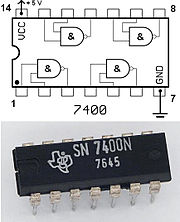
\includegraphics[width=1.5in]{7400}}
\begin{center}
\begin{tabular}{c c c}
\begin{circuitikz}\draw (0,0) node[nand port] (l) {};\end{circuitikz} & \begin{circuitikz}\draw (0,0) node[nor port] (l) {};\end{circuitikz} & \begin{circuitikz}\draw (0,0) node[xnor port] (l) {};\end{circuitikz}\\
NAND & NOR & XNOR
\end{tabular}
\end{center}

Circuits are created by cascading these gates, using the output of one gate as the input for another.
\begin{center}
\begin{circuitikz} \draw
(0,2) node[and port] (myand1) {}
(0,0) node[or port] (myand2) {}
(2,1) node[xnor port] (myxnor) {}
(myand1.out) -- (myxnor.in 1)
(myand2.out) -- (myxnor.in 2);
\end{circuitikz}
\end{center}
These circuits form complex logical statements, and scale up to control the logic behind every computer function.
\end{proc}
\vfill
\pagebreak

\subsection{Combining Operations}
As you may imagine, we can describe longer compound statements by using multiple operations.  For instance, a university might advertise a scholarship by saying that ``a student is eligible if he/she has completed at least two years of college-level work and he/she has at least a 3.0 GPA or he/she has worked full-time for at least five years.''

Let's take a look at this statement; first, define $p$, $q$, and $r$ to represent the simple pieces that are connected by the operations:
\begin{align*}
p &: \textrm{``he/she has completed at least two years of college-level work''}\\
q &: \textrm{``he/she has at least a 3.0 GPA''}\\
r &: \textrm{``he/she has worked full-time for at least five years''}
\end{align*}

Next, try to write the compound statement using the notation we've introduced so far:
\[p \wedge q \vee r\]

There's a problem with this, though; there is some ambiguity in the way the statement is phrased.  Does it mean that a student is eligible after completing two years of college with a 3.0 GPA or after working for five years (with no GPA requirement)?  Or does it mean that the student is eligible after completing two years of college, as long as they EITHER have a 3.0 GPA OR have worked at least five years?

To handle this ambiguity, we can use parentheses to group statements together.  This works like the order of operations in algebra; the parentheses tell us in what order to combine the simple statements.

In this example, if we wanted to make it clear that the first option is the correct one (a student is eligible after completing two years of college with a 3.0 GPA or after working for five years (with no GPA requirement)) we would group the first two statements together:
\[(p \wedge q) \vee r\]

\paragraph{Evaluating Statements with Multiple Operations}
Suppose we want to take the compound statement above and consider a specific case, whether a specific student meets the minimum requirements for the scholarship.  All we have to know is whether $p$, $q$, and $r$ are true for this student.  Then, if we substitute these values into the compound statement and get a true result, the student meets the requirements; if not, the student does not meet the requirements.

For instance, suppose a student applies who has completed two years of college and has five years of work experience, but only had a 2.5 GPA.  For this student, $p$ is true, $q$ is false, and $r$ is true.  If we substitute these values into the compound statement, we have
\[(T \wedge F) \vee T\]
Now we can simplify this statement: the parentheses define the order in which we do so:
\begin{align*}
(T \wedge F) &\vee T\marginnote{F $\wedge$ T $=$ F}\\
F &\vee T\marginnote{F $\vee$ T $=$ T}\\
T
\end{align*}
For this student, the compound statement simplifies to T, so they meet the requirements.
\pagebreak

\begin{example}[https://www.youtube.com/watch?v=TbDIeFHMS00]{Evaluating Statements}
Evaluate the statement $\sim p \wedge q$ when $p$ is true and $q$ is true.

\sol
Substitute these truth values for $p$ and $q$, and start by simplifying $\sim p$:
\begin{align*}
\sim T &\wedge T\marginnote{$\sim T = F$}\\
F &\wedge T\marginnote{$F \wedge T = F$}\\
F
\end{align*}
Thus, when $p$ and $q$ are both true, $\sim p \wedge q$ is false.
\end{example}

\begin{try}
Evaluate the statement $\sim (p \vee q)$ when $p$ and $q$ are both false.
\end{try}

\paragraph{Truth Tables for Statements with Multiple Operations}
We could repeat the substitution and simplification process shown above every time we encounter a new student applying for the scholarship, but it will be more efficient in the long run to simply account for all the possibilities for the students that could apply; this is precisely what a truth table does for us.

Let's practice with the same example, using the compound statement
\[(p \wedge q) \vee r\]
Since we have three simple statements ($p$, $q$, and $r$) we'll need eight rows to account for all possible combinations of truth values.
\begin{center}
\begin{tabular}{|c c c c|}
\hline
$p$ & $q$ & $r$ & $\ldots$\\
\hline
& & &\\
T & T & T & $\ldots$\\
T & F & T & $\ldots$\\
F & T & T & $\ldots$\\
F & F & T & $\ldots$\\
T & T & F & $\ldots$\\
T & F & F & $\ldots$\\
F & T & F & $\ldots$\\
F & F & F & $\ldots$\\
\hline
\end{tabular}
\end{center}

Now, to build up to $(p \wedge q) \vee r$, we'll start by including a column for $p \wedge q$, using the rule for AND to create this column.  Then we'll add another column that combines this new column with $r$ using the rule for OR.  That final column will be the one we're interested in.
\begin{center}
\begin{tabular}{|c c c c c|}
\hline
$p$ & $q$ & $r$ & $p \wedge q$ & $(p \wedge q) \vee r$\\
\hline
& & & &\\
T & T & T & T & T\\
T & F & T & F & T\\
F & T & T & F & T\\
F & F & T & F & T\\
T & T & F & T & T\\
T & F & F & F & F\\
F & T & F & F & F\\
F & F & F & F & F\\
\hline
\end{tabular}
\end{center}
This table lists every possible combination of $p$, $q$, and $r$, and the result for $(p \wedge q) \vee r$ in that case.  If we were sorting applications for this scholarship, we could look at every student and see which row of this truth table they fit into; if it is one of the first five, they are eligible, but if it is one of the last three, they are ineligible.  In reality, we'd probably write a computer program to do the sorting for us, but we'd need to be aware of this logic in order to write that program.
\pagebreak

\begin{example}[https://www.youtube.com/watch?v=cIO6rLWEruw]{Constructing a Truth Table}
Construct the truth table for $\sim p\ \wedge \sim q$.

\sol
In this case, there are only two simple statements ($p$ and $q$), so our truth table will only need four rows to account for all the possibilities.
\begin{center}
\begin{tabular}{|c c c|}
\hline
$p$ & $q$ & $\ldots$\\
\hline
& &\\
T & T & $\ldots$\\
T & F & $\ldots$\\
F & T & $\ldots$\\
F & F & $\ldots$\\
\hline
\end{tabular}
\end{center}

Next, we'll need columns for $\sim p$ and $\sim q$, which will simply invert $p$ and $q$:
\begin{center}
\begin{tabular}{|c c c c c|}
\hline
$p$ & $q$ & $\sim p$ & $\sim q$ & $\ldots$\\
\hline
& & & &\\
T & T & F & F & $\ldots$\\
T & F & F & T & $\ldots$\\
F & T & T & F & $\ldots$\\
F & F & T & T & $\ldots$\\
\hline
\end{tabular}
\end{center}

Finally, we'll combine the columns for $\sim p$ and $\sim q$ using the rule for $\wedge$:
\begin{center}
{\color{green!30!black}
\begin{tabular}{|c c c c c|}
\hline
$p$ & $q$ & $\sim p$ & $\sim q$ & $\sim p\ \wedge \sim q$\\
\hline
& & & &\\
T & T & F & F & F\\
T & F & F & T & F\\
F & T & T & F & F\\
F & F & T & T & T\\
\hline
\end{tabular}}
\end{center}
\end{example}

\begin{try}
Fill in the truth table below for the statement $p\ \vee \sim q$.
\begin{center}
\begin{tabular}{|c c c c|}
\hline
$p$ & $q$ & $\sim q$ & $p\ \vee \sim q$\\
\hline
& & &\\
T & T & & \\
T & F & & \\
F & T & & \\
F & F & & \\
\hline
\end{tabular}
\end{center}
\end{try}

Notice that we could have built the truth table in the last example without using the intermediate rows for $\sim p$ and $\sim q$; to do so, we could substitute each combination of $p$ and $q$ into the final statement $\sim p\ \wedge \sim q$ to jump straight from the first two columns to the final column:
\paragraph{If $p$ is true and $q$ is true:}
\begin{align*}
\sim T\ &\wedge \sim T\\
F\ &\wedge F\\
F
\end{align*}
Therefore, in the row where $p$ is T and $q$ is T, the compound statement $\sim p\ \wedge \sim q$ is F.  The other rows can be done similarly.

The reason we tend to build truth tables as shown in the example above--by slowly adding columns and only performing one operation per column--is that this systematic approach tends to be simpler and avoid errors.
\pagebreak
\text{}
\vfill

\begin{example}[https://www.youtube.com/watch?v=nzBClGWo8Po]{Constructing a Truth Table}
Construct the truth table for the statement $\sim (p \vee q)$.

\sol
Again, we are only dealing with two statements $p$ and $q$, so we begin with the same two columns as before.
\begin{center}
\begin{tabular}{|c c c|}
\hline
$p$ & $q$ & $\ldots$\\
\hline
& &\\
T & T & $\ldots$\\
T & F & $\ldots$\\
F & T & $\ldots$\\
F & F & $\ldots$\\
\hline
\end{tabular}
\end{center}

Next we add a column for $p\ \vee q$.  Note that we're using the parentheses as a guide for the order; since the parentheses group the $p\ \vee q$, we'll fill in that column first, then negate it.
\begin{center}
\begin{tabular}{|c c c c|}
\hline
$p$ & $q$ & $p\ \vee q$ & $\ldots$\\
\hline
& & &\\
T & T & T & $\ldots$\\
T & F & T & $\ldots$\\
F & T & T & $\ldots$\\
F & F & F & $\ldots$\\
\hline
\end{tabular}
\end{center}

Finally, we negate this last column to get a column for $\sim (p\ \vee q)$.
\begin{center}
{\color{green!30!black}
\begin{tabular}{|c c c c|}
\hline
$p$ & $q$ & $p\ \vee q$ & $\sim (p\ \vee q)$\\
\hline
& & &\\
T & T & T & F\\
T & F & T & F\\
F & T & T & F\\
F & F & F & T\\
\hline
\end{tabular}}
\end{center}
\end{example}
\vfill

Notice that the column for $\sim (p\ \vee q)$ here is identical to the column for $\sim p\ \wedge \sim q$ in the previous example.  Again, this is no accident; this is another representation of one of De Morgan's laws.
\vfill

\begin{try}
Fill in the truth table below for the statement $\sim p\ \wedge (p\ \vee \sim q)$.
\begin{center}
\begin{tabular}{|c c c c c c|}
\hline
$p$ & $q$ & $\sim p$ & $\sim q$ & $p\ \vee \sim q$ & $\sim p\ \wedge (p\ \vee \sim q)$\\
\hline
& & & & &\\
T & T & & & &\\
T & F & & & &\\
F & T & & & &\\
F & F & & & &\\
\hline
\end{tabular}
\end{center}
\end{try}
\vfill
\text{}
\vfill
\text{}
\vfill
\pagebreak

\begin{example}[https://www.youtube.com/watch?v=Sdh658OUmFk]{Constructing a Truth Table}
Construct the truth table for the statement $(p\ \wedge \sim q)\ \vee (r\ \wedge \sim p)$.

\sol
Now we have three pieces ($p$, $q$, and $r$), so we'll need three starting columns and eight rows to account for all the possibilities.
\begin{center}
\begin{tabular}{|c c c c|}
\hline
$p$ & $q$ & $r$ & $\ldots$\\
\hline
& & &\\
T & T & T & $\ldots$\\
T & F & T & $\ldots$\\
F & T & T & $\ldots$\\
F & F & T & $\ldots$\\
T & T & F & $\ldots$\\
T & F & F & $\ldots$\\
F & T & F & $\ldots$\\
F & F & F & $\ldots$\\
\hline
\end{tabular}
\end{center}

Next, we'll need $\sim p$ and $\sim q$ in the final statement, so we'll add a column for each of those.
\begin{center}
\begin{tabular}{|c c c c c c|}
\hline
$p$ & $q$ & $r$ & $\sim p$ & $\sim q$ & $\ldots$\\
\hline
& & & & &\\
T & T & T & F & F & $\ldots$\\
T & F & T & F & T & $\ldots$\\
F & T & T & T & F & $\ldots$\\
F & F & T & T & T & $\ldots$\\
T & T & F & F & F & $\ldots$\\
T & F & F & F & T & $\ldots$\\
F & T & F & T & F & $\ldots$\\
F & F & F & T & T & $\ldots$\\
\hline
\end{tabular}
\end{center}

Next, add two more columns: one for $p\ \wedge \sim q$ and one for $r\ \wedge \sim p$.  The last step will be to combine these two columns with $\vee$.
\begin{center}
\begin{tabular}{|c c c c c c c c|}
\hline
$p$ & $q$ & $r$ & $\sim p$ & $\sim q$ & $p\ \wedge \sim q$ & $r\ \wedge \sim p$ & $\ldots$\\
\hline
& & & & & & &\\
T & T & T & F & F & F & F & $\ldots$\\
T & F & T & F & T & T & F & $\ldots$\\
F & T & T & T & F & F & T & $\ldots$\\
F & F & T & T & T & F & T & $\ldots$\\
T & T & F & F & F & F & F & $\ldots$\\
T & F & F & F & T & T & F & $\ldots$\\
F & T & F & T & F & F & F & $\ldots$\\
F & F & F & T & T & F & F & $\ldots$\\
\hline
\end{tabular}
\end{center}

Finally, combine these last two columns with the OR rule.
\begin{center}
{\color{green!30!black}
\begin{tabular}{|c c c c c c c c|}
\hline
$p$ & $q$ & $r$ & $\sim p$ & $\sim q$ & $p\ \wedge \sim q$ & $r\ \wedge \sim p$ & $(p\ \wedge \sim q)\ \vee (r\ \wedge \sim p)$\\
\hline
& & & & & & &\\
T & T & T & F & F & F & F & F\\
T & F & T & F & T & T & F & T\\
F & T & T & T & F & F & T & T\\
F & F & T & T & T & F & T & T\\
T & T & F & F & F & F & F & F\\
T & F & F & F & T & T & F & T\\
F & T & F & T & F & F & F & F\\
F & F & F & T & T & F & F & F\\
\hline
\end{tabular}}
\end{center}
\end{example}
\vfill
\pagebreak

\subsection{Quantified Statements}
Some statements only make a claim about a specific category.  For instance, one might say that ``all politicians are dishonest.''  In this case, only those who fall into the category of politician are considered.  This is an example of a \textbf{quantified statement}. 

The words ``all'' or ``some'' (similarly ``none'' or ``not all'') are called \textbf{quantifiers}, since they refer to quantities, limiting the scope of a statement to a given category.

\begin{formula}{Quantifiers}
\paragraph{The Universal Quantifier} \text{}

The universal quantifier refers to \textbf{all} of a given category.  The symbol $\forall$\marginnote{($\forall$ is an upside-down A)} is used to mean ``for all.''\\

\paragraph{Ex:} To\marginnote{Note: ``none'' is a variation of ``for all.''  For instance, ``no pig is beautiful'' could be written ``$\forall p$ such that $p$ is a pig, $p$ is not beautiful.''} say that all human beings are mortal, we could write
\begin{center}
``$\forall$ human beings $x$, $x$ is mortal'' or\\
``$\forall x$ such that $x$ is a human being, $x$ is mortal''
\end{center}
\vspace{0.1in}

\paragraph{The Existential Quantifier} \text{}

The existential quantifier refers to \textbf{some} of a given category.  The symbol $\exists$\marginnote{($\exists$ is a backwards E)} is used to mean ``there exists.''  This is equivalent to saying that ``there is at least one.''\\

\paragraph{Ex:} To say that some dogs are retrievers, we could write
\begin{center}
``$\exists x$ such that $x$ is a dog and $x$ is a retriever''
\end{center}
\end{formula}

We can draw diagrams to represent quantified statements, like the following examples.  We'll use circles to represent categories, but the size of the circles is not relevant; we're only interested in the location and interaction of the circles.

\begin{example}[https://www.youtube.com/watch?v=y1Rm8lB3fzw]{Diagram for the Universal Quantifier}
Draw a diagram to represent the statement that ``all battleships are ships.''

\sol
The diagram below looks like a Venn diagram.  The outer circle represents all ships, and the inner circle represents battleships.

\begin{center}
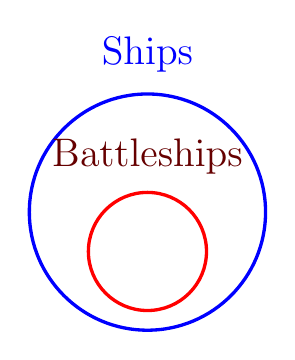
\begin{tikzpicture}
  %\draw [very thick,color=orange!30!black, fill=orange!20] (-3cm,-2cm) rectangle (3cm,2.6cm);

  \draw [very thick,color=blue, fill=white] (0,0) circle (1.5cm);
  \draw [yshift=2cm,xshift=0cm] node {\color{blue}\Large Ships};
  
  \draw [very thick,color=red, fill=white] (0,-0.5) circle (0.75cm);
  \draw [yshift=0.7cm,xshift=0cm] node {\color{red!40!black}\Large Battleships};
  
  
\end{tikzpicture}
\end{center}

Notice that anything in the battleship category is also automatically in the ship category; hence, this represents the quantified statement that ``all battleships are ships.''
\end{example}
\pagebreak

\begin{example}[https://www.youtube.com/watch?v=m21zOUD-c4w]{Diagram for the Existential Quantifier}
Draw a diagram to represent the statement that ``some clouds are white.''

\sol
Now, the left circle represents all white things, and the right circle represents all clouds.

\begin{center}
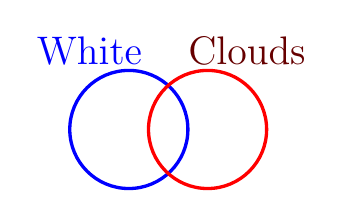
\begin{tikzpicture}
  %\draw [very thick,color=orange!30!black, fill=orange!20] (-3cm,-2cm) rectangle (3cm,2.6cm);

  \draw [very thick,color=blue] (-0.5,0) circle (0.75cm);
  \draw [yshift=1cm,xshift=-1cm] node {\color{blue}\Large White};
  
  \draw [very thick,color=red] (0.5,0) circle (0.75cm);
  \draw [yshift=1cm,xshift=1cm] node {\color{red!40!black}\Large Clouds};
  
  
\end{tikzpicture}
\end{center}

Notice that there is some overlap, which is the clouds that are white.  However, there are things that are white that are not clouds (Paper! Snow! A ghost!) and some clouds that are not white.  This diagram therefore accurately represents the statement that ``some clouds are white.''
\end{example}

\subsection{Negating Quantified Statements}
Negating a quantified statement is not initially an intuitive process.  For instance, suppose we have a false statement like ``all clouds are white.''  If we negate it, we should get a true statement.

You may be tempted to write the negation as ``all clouds are not white.''  However, this too is a false statement, so it cannot be the negation of the first false statement.

The correct negation would be ``NOT all clouds are white,'' which can also be written ``some clouds are not white'' or ``there is at least one cloud that is not white.''

\begin{formula}{Negating a Quantified Statement}
The negation of the statement ``all $A$ are $B$'' is ``some $A$ are not $B$.''

The negation of the statement ``some $A$ are $B$'' is ``all $A$ are not $B$.''
\end{formula}

\begin{example}[https://www.youtube.com/watch?v=ro0-8GznkW0]{Negating Quantified Statements}
Write the negation of each of the following quantified statements:
\begin{enumerate}[(a)]
\item All vegetarians eat carrots
\item Some birds are flightless
\item Every car salesman is dishonest
\item There are some foods that cause cancer
\end{enumerate}

\sol
\begin{enumerate}[(a)]
\item \emph{Some vegetarians do not eat carrots}

\item \emph{All birds are not flightless} OR \emph{No birds are flightless} OR \emph{All birds can fly}

\item \emph{At least one car salesman is not dishonest}

\item \emph{No foods cause cancer}
\end{enumerate}

Notice that there can be several equivalent ways to phrase something in English that all correspond to the same logical statement.
\end{example}

\begin{try}
Write the negation of the statement ``All dogs go to heaven.''
%%% POSSIBLE ANSWERS:
%\begin{enumerate}[(a)]
%\item All dogs don't go to heaven.
%\item Some dogs go to heaven.
%\item There are some dogs that don't go to heaven.
%\item There is no dog that doesn't go to heaven.
%\end{enumerate}
\end{try}